\chapter{Technologia CUDA}
\section{Współbieżna przyszłość}
Kiedy w roku 2005 H. Sutter \cite{lunch} opublikował artykuł o intrygująco brzmiącej nazwie 'Koniec darmowego lanczu', w szeroko pojętym środowisku deweloperskim rozgorzała dyskusja. Autor przedstawił, że obserwujemy kres wykładniczego wzrostu wydajności mikroprocesorów, rozumianego przez wzrost częstotliwości taktowania ich zegarów czy ilości możliwych do wykonania operacji mierzonych w GFLOP/S-ach. Z tym argumentem, nie można się nie zgodzić patrząc na oferowane na rynku procesory firmy Intel przedstawione na rys \ref{proce}.

\begin{figure}[ht]
\centering
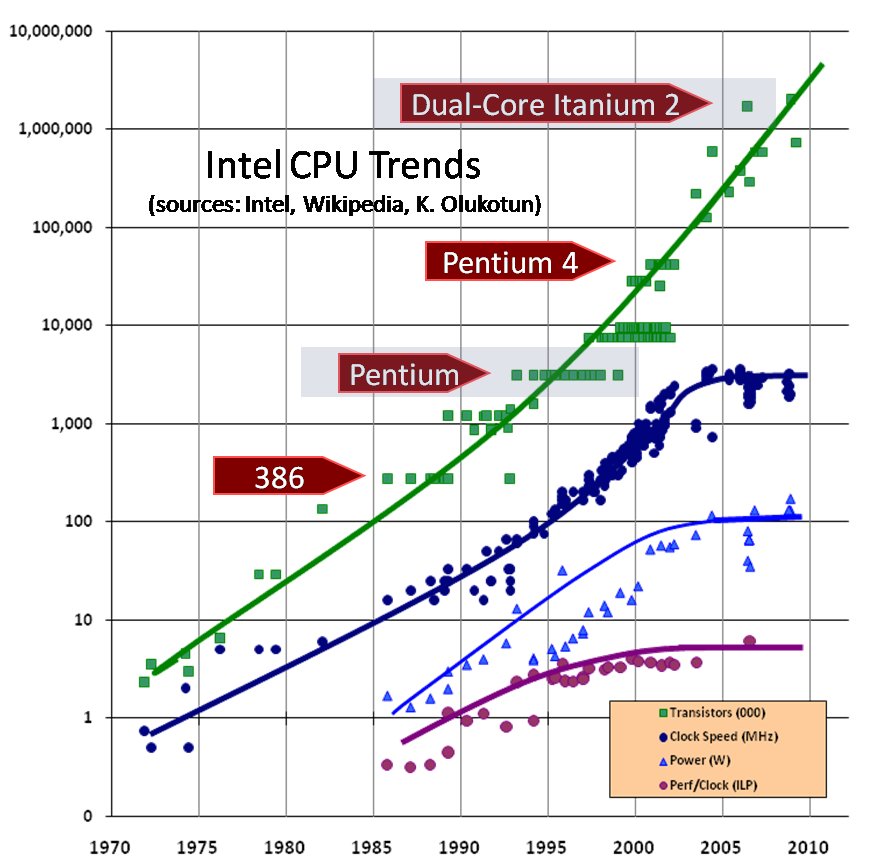
\includegraphics[scale=1.0]{images/CPU.png}
\caption{.  Źródło: http://www.gotw.ca/}
\label{proce}
\end{figure}

Ważniejszą jednak tezą postawioną przez Suttera było stwierdzenie, że programiści nie będą mogli dłużej korzystać ze wzrostu mocy obliczeniowej sprzętu. Taki wzrost wydajności często okazywał się dla twórców aplikacji niezastąpiony. Napotykając problemy wydajnościowe w swoim oprogramowania programiści mogli albo poświęcić się żmudnemu procesowi optymalizacji, albo poprostu podnieść jej wymaganie sprzętowe. Często, głównie ze względów ekonomicznych drugi wariant było wybierany, gdyż ograniczał się do tylko do poczekania nowe generacje sprzętu. To zjawisko, ciekawie scharakteryzował J. Spolsky przytaczany w \cite{nolunch} ,,Jako programista masz wybór, albo spędzisz pół roku na przedesignowaniu swojej aplikacji, wstawiając kod asemblera w krytycznych sekcjach, albo na wakacjach, grając na perkusji w rockowej kapeli. Niezależnie od alternatywy którą wybierzesz, twoja aplikacji będzie działała szybciej,,.

Czy jednak założenie o niskim wzroście wydajności współczesnym mikroprocesorów jest prawdziwe? Wprawdzie częstotliwość taktowania nie podlega już takim trendom co wcześniej, jednak dzisiejsze architektury CPU oferują więcej niż jeden rdzeni zdolnych do wykonywania programu. Obecnie na rynku jest już oferowany procesor Intel z serii i7, który może posiadać do 8 fizycznych rdzeni. Dodatkowo, nowe technologie takie jak hyperthreading, pipelining czy zaawansowany brach prediction pozwalają na możliwie szybkie, czy wręcz równoległe wykonywanie fragmentów sekwencyjnego kodu.

Mimo nowoczesnej architektury CPU, sekwencyjnie programy i tak wykonywane są tylko na pojedynczym rdzeniu\cite{massive}, który jak było to opisane wcześniej, na przestrzeni ostatnich lat stał się znacząco szybszy. Nawet najbardziej zaawansowane heurystyki stosowane w dzisiejszych kompilatorach nie są w stanie zamienić sekwencyjnego kodu w wydajny kod zrównoleglony. 

Sutter stwierdza, że odpowiedzą na postawiony wyżej problem jest zmiana paradygmatu z programowania sekwencyjnego na współbieżne. Tworzone wielowątkowe aplikacje będą w stanie korzystać z wielordzeniowych architektur, co przyspieszy ich wykonywanie a programistom pozwoli nadal oczekiwać na ,,darmowy lancz''. Samo jednak przejście nie będzie łatwe, przyjemne, a przede wszystkim tanie. Wg Suttera taka zmiana wiązać się będzie nie tylko ze zmianą architektury aplikacji, lecz też systemu operacyjnego czy konstrukcjami języków programowania. 

Zmiany w stronę wielowątkowości obserwowane są jakiegoś czasu. W nowym standardzie języka C++ 11, biblioteka obsługująca wątki będzie wchodzić w skład biblioteki standardowej, Microsoft publikuje wielowątkowe wersje popularnych bibliotek dla Platformy .NET jak PLINQ, a NVIDIA biblioteki algorytmiczne (CUFFT) wykonywane na GPU. Marsz w stronę wielowątkowości obserwujemy cały czas, ale nie będzie to jednak rewolucja zapowiadana w \cite{rewolucja}, lecz moim zdaniem bardziej ewolucja. Warto dodać, że dużo pracy zostało już wykonane. Serwery www oraz bazy danych są świetnym przykładem wielowątkowych aplikacji.

Koleją istotną kwestią w projektowaniu wielowątkowych aplikacji jest jej skalowalność. Jeżeli dany problem programistyczny nie będzie w stanie być dynamicznie dzielony na podproblemy, które będą mógły być rozwiązany indywidualnie, korzyści związane z przyrostem ilości rdzeni w sprzęcie nie będą zauważane. Taki podział często okazuje się być nietrywialny, a czasem niemożliwy. Nie można też oczekiwać wielkich wzrostów wydajności, ponieważ nie cały kod aplikacji może być zrównoleglony. Dobrze opisuje to formuła stworzona w 1967 r. przez G. Amdahl.

\begin{equation}
W(N) = \frac{1}{(1-S) + \frac{S}{N}}
\end{equation}
,gdzie $N$ jest ilością jednostek wykonywania, a $S$ jest \% kodu programu, który może być zrównoleglony. I tak dla 8 rdzeni i programu i współczynnika $S=60\%$ otrzymujemy wzrost wydajności około 2.1 raza.

Współbieżność jest bez wątpienia problemem z którym każdemu programiście przyjdzie się kiedyś zmierzyć. Możliwe, że do niektórych problemów wystarczą mu gotowe rozwiązania z dostępnych bibliotek, jednak myślenie o problemie i przedstawienie go w postaci dającej się zrównoleglić będzie rzeczą najważniejszą. Środowiska naukowe pomagają w tym aspekcie bardzo istotnie. Każdego roku publikowane są artykuły przedstawiające często nowatorskie podejścia do zagadnieñ wskazując możliwość ich współbieżnego rozwiązania. Oczekuję, że w następnych latach trend z programowaniem równoległym będzie przybierał na sile, czego owocem będą nowe, innowacyjne metody i technologie.

\section{Powstanie CUDA}

Technologia CUDA (Compute Unified Device Architecture) została po raz pierwszy zaprezentowana przez NVIDIA w listopadzie 2006 r. Przedstawiła ona nowy model programowania aplikacji w którym sekwencyjne fragmenty kodu są wykonywane na CPU, natomiast te wymagające obliczeniowo, na procesorach graficznych (GPU). Pierwsze karty graficzne z serii GeForce 8800, implementujące technologię CUDA, pojawiły się w roku 2006 r. Programiści od tego czasu mogą korzystać ze specjalnie zaprojektowanych w tym celów interfejsów programistycznych bibliotek CUDA.

Sama koncepcja programowania procesorów graficznych jest znana od dawna. Programiści używając interfejsów do programowania shaderów, dostępnych chociażby w OpenGL 1.4 (2002) czy Direct3D 8.0 (2001), mogli dokonywać równoległych obliczeñ na kartach graficznych. Wymagało to jednak często wielu trików, takich jak przekazywanie danych poprzez tekstury czy odczytywania danych wyjściowych z wygenerowanej ramki obrazu. NVIDIA wyszła naprzeciw tym problemom, tworząc dedykowane na ten cel interfejsy programistyczne napisane w C i C++.

Na sukces technologi CUDA złożyło się wg \cite{massive} parę czynników. Pierwszym jest fakt, że programiści aplikacji równoległych otrzymali środowisko w którym ich kod, wg zapewnieñ NVIDIA, będzie wykonywany poprawnie, niezależnie od używanego sprzętu. Ma to szczególnie ważne znaczenie, biorąc pod uwagę fakt, że projektanci kart graficznych nie zakładali początkowo ich użycia do obliczeñ inżynierskich. I tak np. kalkulacje na liczbach zmiennoprzecinkowych na różnych kartach graficznych NVIDIA do 2006 r. mogły skutkować innymi wynikami. Dopiero specyfikacja technologii CUDA wymusiła na projektantach sprzętu zgodność ze standardami publikowanymi przez IEEE.

Kolejnym czynnikiem, który zdecydował o sukcesie technologii CUDA jest dostępność medium, na którym wielowątkowe, zrównoleglone aplikacje mogą być wykonywane. W chwili obecnej na rynku znajdują się setki milionów kart graficznych wyprodukowanych przez NVIDIA zdolnych do wykonania kodu napisanego w CUDA. Ma to bardzo istotny wymiar ekonomiczny, ponieważ wiele specjalistycznych (np. w medycynie) aplikacji nie musi być więcej dostarczana z drogim, dedykowanym dla tego celu sprzętem. Spowodowało to zatem wzrost rynku dla tego typu rozwiązañ i stworzyło ekonomiczne uzasadnienie do dalszej pracy nad współbieżnie wykonywanymi aplikacjami.

Ostatnim, najbardziej oczywistym czynnikiem, jest wzrost wydajności. Procesory graficzne składające się z multiprocesorów strumieniowych są przystosowane do przetwarzania dużej ilośći danych jednocześnie. W nowych architekturach takich jak GeForce z serii 680 posiadającą aż 1536 rdzeni zdolnych do równoległego wykonywania kodu. Efektem tego może być wzrost wydajności aplikacji w niektórych zastosowaniach nawet do 150 razy \cite{prez}.

\section{Model programowania}

Zaproponowany we frameworku CUDA model programowania zakłada możliwość skompilowania kodu w dwóch różnych kontekstach - na CPU (host) oraz GPU (device). Jako kontekst rozumiany jest specyficzny dla danej architektury zestaw instrukcji dla procesora. Fragmenty programu, których zrównoleglenie jest niemożliwe są tworzone w kontekście hosta, natomiast te wymagające intensywnych, wielowątkowych obliczeñ w kontekście device'a. Współistnienie dwóch konteksów w jednym programie wykonywanlym możliwe jest dzięki zestawie bibliotek i narzędzi dostarczanych wraz z pakietem CUDA. Z punktu widzenia programisty zmiana kontekstu ogranicza się do wykonania specyficznego rodzaju funkcji, nazywanego w nomenklaturze CUDA kernelami.

Skompilowanie kodu dla karty graficznej możliwe jest za pomocą dostarczanego przez NVIDIA kompilatora nvcc. Kod Źródłowy dla nvcc jest najczęściej napisany w ANSI C z rozszerzeniami. Możliwe jest jednak pisanie kodu urządzenia w innych językach programowania takich jak C++, Fortran, Java czy Python. 

\begin{figure}[ht]
\centering
\tikzstyle{layer}=[rounded corners=10pt,shading=center]

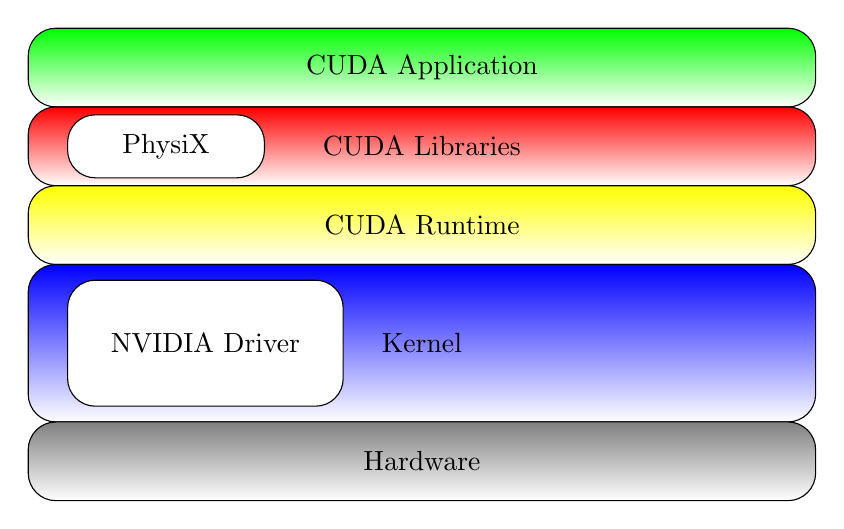
\begin{tikzpicture}
\draw[style=layer,top color=green] (0,0) rectangle (10,1) node[pos=0.5] {CUDA Application};
\draw[style=layer,top color=red] (0,-1) rectangle (10,0) node[pos=0.5] {CUDA
	Libraries};
\draw[style=layer,top color=white] (0.5,-0.9) rectangle (3,-0.1) node[pos=0.5]
{PhysiX};
\draw[style=layer,top color=yellow] (0,-2) rectangle (10,-1) node[pos=0.5] {CUDA
	Runtime};
\draw[style=layer,top color=blue] (0,-4) rectangle (10,-2) node[pos=0.5] {Kernel};
\draw[style=layer,top color=white] (0.5,-3.8) rectangle (4,-2.2) node[pos=0.5]{NVIDIA Driver};
\draw[style=layer,top color=gray] (0.0,-5) rectangle (10,-4) node[pos=0.5]{Hardware};

\end{tikzpicture}

\caption{CUDA}
\label{cuda-model}
\end{figure}

\section{GPU}

\begin{figure}[ht]
\centering
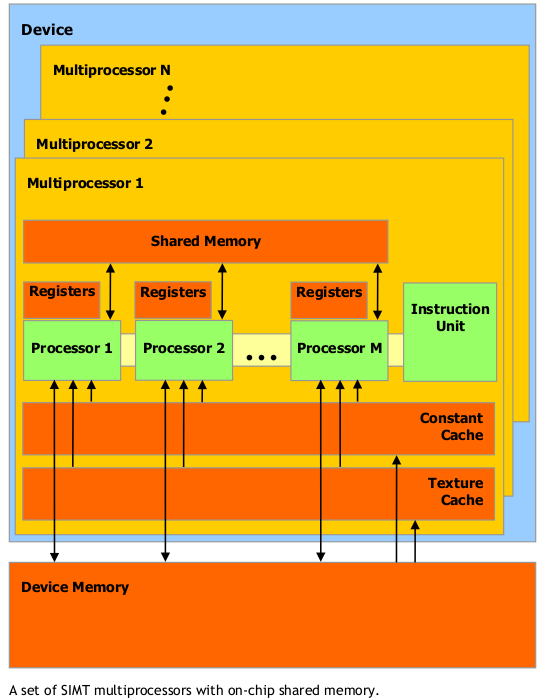
\includegraphics[scale=0.8]{images/gpu.png}
\caption{.  Źródło: CUDA Manual}
\label{proce}
\end{figure}



